% !TeX spellcheck = en_US
\section{Neural Network Architecture}
In the evolving landscape of NLP, the adaptation of Convolutional Neural Networks on various domains of processing and classification, has marked a significant technological advancement. This transition underscores the versatility of CNNs, which, despite their visual data origins, excel in deciphering the intricate patterns of textual information. The project in discussion exemplifies this innovative application, employing a CNN to tackle a multiclass text classification challenge. Herein, we delve into the architectural choices and strategic decisions underlying the model's design, offering a comprehensive understanding of its construction and functionality. \\
A universal question is wether we must use CNN's or RNN's. The choice between a Convolutional Neural Network (CNN) and a Recurrent Neural Network (RNN) depends on the specific task and the nature of our data. \\

In general, RNN is a class of artificial neural network where connections between nodes form a directed graph along a sequence. It is basically a sequence of neural network blocks that are linked to each other like a chain. Each one is passing a message to a successor. This architecture allows RNN to exhibit temporal behavior and capture sequential data which makes it a more ‘natural’ approach when dealing with textual data since text is naturally sequential. RNNs usually are good at predicting what comes next in a sequence\\

Controversely, CNN is a class of deep, feed-forward artificial neural networks where connections between nodes do not form a circle. CNNs are basically just several layers of convolutions with nonlinear activation functions like ReLU or tanh applied to the results. In a traditional feedforward neural network we connect each input neuron to each output neuron in the next layer. That’s also called a fully connected layer. In CNNs we don’t do that. Instead, we use convolutions over the input layer to compute the output. This results in local connections, where each region of the input is connected to a neuron in the output. Each layer applies different filters, typically hundreds or thousands like the ones shown below, and combines their results. CNNs can learn to classify a sentence or a paragraph.\\

An RNN is trained to recognize patterns across time, while a CNN learns to recognize patterns across space. The best way to determine which to use is to try both and see which one performs better on our project. \\
A big argument for CNNs is that they are exceptionaly fast. Based on computation time, CNN's seems to be much faster, sometimes also 5 times faster, than RNN's.

\begin{figure}[htpb]
	\centering
	\begin{subfigure}{0.47\linewidth}
		\centering
		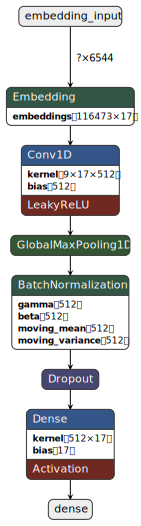
\includegraphics[height=0.9\textheight]{Images/model_level_1.keras.pdf}
		\caption{\textit{category\_level\_1}}
	\end{subfigure}
	\begin{subfigure}{0.47\linewidth}
		\centering
		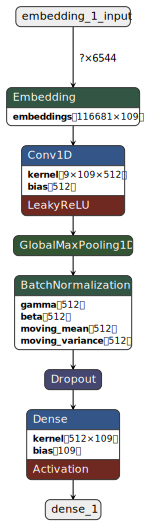
\includegraphics[height=0.9\textheight]{Images/model_level_2.keras.pdf}
		\caption{\textit{category\_level\_2}}
	\end{subfigure}
	\caption{Architecture of the neural networks}
	\label{fig:nn_architectures}
\end{figure}
 
%\begin{minipage}{0.47\linewidth}
%	\centering
%	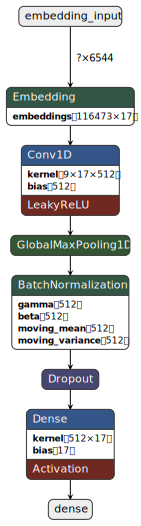
\includegraphics[height=0.9\textheight]{Images/model_level_1.keras.pdf}
%	\captionof{figure}{Architecture of the model for \textit{category\_level\_1}}
%\end{minipage}\hfill
%\begin{minipage}{0.48\linewidth}
%	\centering
%	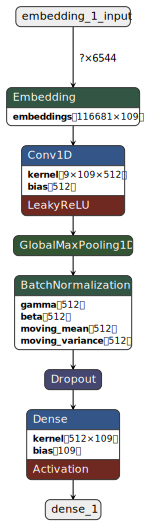
\includegraphics[height=0.9\textheight]{Images/model_level_2.keras.pdf}
%	\captionof{figure}{Architecture of the model for \textit{category\_level\_2}}
%\end{minipage}

\subsection{Embedding Layer}
The embedding layer is a critical component in the neural network architecture, serving as the foundational layer that deals directly with the text input. In the general context of NLP and deep learning, an embedding layer effectively translates tokenized and sequenced text data into dense vectors of fixed size. This layer maps each word to a high-dimensional space where words with similar meanings are located in proximity to one another, thereby capturing semantic relationships in a way that is not possible with sparse representations such as one-hot encoding.

From Figure~\ref{fig:nn_architectures}, we can see that embedding layer has been configured with a vocabulary size of $\num{129865}$ and an output dimension of $17$ for \verb|category_level_1| and of $109$ for \verb|category_level_2|. Those numbers are not set by a random factor, but they represent the number of unique labels in each category. By applying this very specific number (\textit{which changes with different input}), we are sure that our model will compute the correct probability distribution output for the given input data. This setup suggests that our model is designed to handle a large corpus with a rich vocabulary, transforming each token into a $x$-dimensional vector. The decision to use such an embedding size balances the need for a nuanced representation of the input text against the computational efficiency of the model. A smaller dimensionality in the embedding space ensures that the model remains computationally tractable, while still allowing for a meaningful representation of words.

\begin{wrapfigure}{r}{0.4\linewidth}
	\centering
	\includegraphics[width=\linewidth]{Images/embedding_visualize.png}
	\caption{Visualization of an embedding layer}
\end{wrapfigure}

Moreover, the embedding layer is paramount when working with sequences of different lengths. After tokenizing, padding, and converting texts into sequences, the embedding layer takes these sequences as input and provides a uniform output shape, which is essential for the subsequent convolutional layers to function correctly. Unlike one-hot encoded vectors that are sparse and high-dimensional, the dense embeddings can capture more information in a lower-dimensional space.

Thus, by choosing to implement an embedding layer, our model is able to learn an internal representation for the words in the dataset during training. This is advantageous over using pre-trained embeddings when the text data has unique contextual meanings or when the domain-specific vocabulary may not be well-represented by pre-trained word vectors. It allows the model to adapt the word representations to the nuances of the specific dataset and task at hand.

Below is the code we wrote to add an embedding layer in our system.
\begin{lstlisting}[language=Python]
model = Sequential()
model.add(Embedding(input_dim=int(num_words), output_dim=labels_unique_num, input_length=input_length))
\end{lstlisting}

\begin{itemize}
	\item Using \verb|Sequential()| in our code means that all layers we will add later are going to be sequential ones.
	\item \verb|Embedding()| is the actual layer that is mentioned above. We can see here that it has as input dimension the total number of \verb|num_words| of the \textit{train} dataset, for output dimension the unique labels number and for input length the maximum sentence length of the dataset.
\end{itemize}

\subsection{Conv1D Layer}
The inclusion of a convolutional layer with a kernel size of $20$ and $512$ filters in the neural network architecture is a calculated choice tailored for the demands of text classification tasks. The kernel size, or filter size, determines the width of the convolution window that scans across the input data. In this case, a kernel size of $20$ allows the model to examine twenty adjacent words at a time, enabling the capture of context within these word sequences. This can be particularly effective for recognizing patterns or features in text that span multiple words, such as phrases or specific syntactic constructions, which are often pivotal for understanding the overall meaning and sentiment of the text.

The use of $512$ filters within this layer significantly increases the model's capacity to extract features. Each filter can be thought of as a feature detector, looking for different types of patterns in the text. With $512$ filters, the network is well-equipped to identify a wide array of textual features, making it robust in the face of the complexity and variability inherent in natural language. This high number of filters is indicative of the model's deep architecture, designed to handle the intricate task of classifying texts into multiple categories, where a nuanced understanding of the language is crucial.

Furthermore, the choice of the \verb|Leaky ReLU| activation function following the convolutional layer adds an element of non-linearity to the model, allowing for more complex relationships to be learned. \verb|LeakyReLU| is particularly chosen over the standard \verb|ReLU| to mitigate the issue of neurons \say{dying} during training; it allows a small, non-zero gradient when the unit is not active, thus maintaining a gradient flow even for neurons that output negative values. This can lead to more efficient learning and better performance, especially in deeper networks that are prone to saturation and dead neurons.
\begin{lstlisting}{language=Python}
model.add(Conv1D(512, 20, activation=LeakyReLU(alpha=0.01)))
\end{lstlisting}
	
\begin{itemize}
	\item \verb|LeakyReLU| is used as activation layer here with $\alpha=0.01$. Initially, we made use of the classic \verb|ReLU| but we wanted to be sure that dead neurons will not be a problem for our case.
\end{itemize}

\subsection{Global Max Pooling 1D}
Pooling is a technique used in the field of neural networks, particularly in CNNs to reduce the spatial dimensions of the input volume for the next layer in the network. It is a form of downsampling that reduces the number of parameters and computation and helps to achieve spatial invariance to input transformations. However, the pooling layer contains no parameters. Instead, pooling operators are deterministic.\\

Pooling layers typically follow Convolutional Layers and come in different types, with Max Pooling being one of the most common. Max pooling is a deterministic pooling operator that calculates the maximum value in each patch of the feature map. Max Pooling helps in making the detection of features somewhat invariant to scale and orientation changes. It also reduces the computational cost by reducing the number of parameters.\\

Nevertheless, the amount of data that we have in this project is huge. So we must find a faster and less complex method to reduce our computations. That is why we are using Global Max Pooling 1D. Global Max Pooling 1D is a specific type of pooling operation designed for 1-dimensional input, such as in the case of time series data or sequences. Unlike the traditional Max Pooling operation that looks at patches of the input volume, Global Max Pooling operates over the entire length of the input data in each dimension and takes the maximum value over the entire dimension. In other words, The role of Global Max Pooling 1D in this context is to capture the most important feature (the highest value) for each feature map across the entire sequence, which can be especially beneficial for identifying key signals in the text for classification purposes.\\
By reducing the output of the convolutional layers from a 3D tensor (batch size, sequence length, features) to a 2D tensor (batch size, features) and by capturing the key features each time, Global Max Pooling reduces overfitting. It reduces overfitting by simplifying the model architecture and focusing on the most important features.\\

\begin{lstlisting}
#Add Global_Max_Pooling Layer
model.add(GlobalMaxPooling1D())
\end{lstlisting}

This snippet of code does exactly what we explained. It is adding a \verb*|GlobalMaxPooling1D| layer to the model. This will reduce the output of the previous layer to its maximum value over the time dimension.


\subsection{Batch Normalization}
Batch Normalization is an excellent layer that significantly lowers our neural network's overall complexity \cite{ioffe2015batch}.
This layer standardizes the inputs to a layer for each mini-batch, stabilizing the learning process. By normalizing the features to have a mean of zero and a standard deviation of one, it ensures that no particular feature dominates the gradient updates during training, which can lead to faster convergence. This is particularly beneficial after pooling layers (\textit{just as we did here}), as the aggregation can sometimes lead to a shift in the distribution of the pooled features.

Moreover, the \verb|BatchNormalization| layer is strategically placed. It is positioned soon following pooling to ensure that activations sent into succeeding layers support good gradient flow and promptly address any potential distribution shifts resulting from the pooling procedure. In this setup, the BatchNormalization layer serves as a regulatory checkpoint in the network, guaranteeing that the feature representations retain favorable attributes that promote effective learning.

\begin{lstlisting}[language=Python]
model.add(BatchNormalization())
\end{lstlisting}
The snippet above just adds a \verb|BatchNormalization| layer from \verb|tensorflow|'s library.

\subsection{Dropout Layer}
The Dropout layer is an essential technique in the training of deep neural networks to prevent overfitting. The term overfitting is used in the context of predictive models that are too specific to the training data set and thus learn the scatter of the data along with it. This often happens when the model has too complex a structure for the underlying data or because certain neurons from different layers influence each other.  The problem then is that the trained model generalizes very poorly, i.e., provides inadequate predictions for new, unseen data. The performance on the training data set, on the other hand, was very good, which is why one could assume a high model quality.\\
With deep neural networks, it can happen that the complex model learns the statistical noise of the training data set and thus delivers good results in training. In the test data set, however, and especially afterwards in the application, this noise is no longer present, and therefore the generalization of the model is very poor.
\\

However, we do not want to abandon the deep and complex architecture of the network, as this is the only way to learn complex relationships and thus solve difficult problems.\\

This is why we are using a Dropout Layer. The Dropout layer combats this by randomly setting a fraction of the input units to zero at each step during training time, which helps to prevent complex co-adaptations on the training data. It forces the network to learn more robust features that are useful in conjunction with various different random subsets of the other neurons.  Thus, they have no influence on the prediction and also in the backpropagation. \\

In our model, adding \verb*|Dropout(0.2)| means that during training. each input to the Dropout Layer has a $20\%$ chance of being set to zero. Generally, the Dropout rate is set as the percent of the test\_data. In our project, we have set \verb*|test_data=0.2|. Equivalently, the \verb*|dropout_rate=0.2|.\\

\begin{lstlisting}
# Add Dropout Layer
model.add(Dropout(0.2))	
\end{lstlisting}

Dropout is one of the most effective and commonly used regularization techniques to achieve good generalization, which is particularly important in a multiclass classification task where the model must discern between multiple different classes based on the input CSV file.
Therefore, the use of a Dropout layer aligns with the overall objective of our project to create a robust and accurate multiclass text classifier by leveraging the strengths of neural networks in handling complex patterns in the data while ensuring that the model's performance is not hindered by overfitting.

\subsection{Dense Layer}
The final stage of our multi-class text classifier incorporates a Dense layer using \verb|softmax| as activation function. As the layer that generates the final predictions, it is the last and most important layer in the network.

The Dense layer, or fully connected layer, is the layer where all neurons from the previous layer are connected to each neuron in the Dense layer. In your model, the Dense layer has a configuration of $512$ units connecting to \verb|labels_unique_num| units, corresponding to the number of unique labels in your classification task. The choice of having that many units suggests that the network is designed to capture a broad and complex representation of the features learned from previous layers. These $512$ units serve as a high-dimensional feature space in which the learned representations from the convolutional and pooling layers are combined and transformed.

Each of these units carries forward the learned patterns to the output layer, which consists of a specified amount of neurons, one for each class. This allows the model to make a decision for each class based on the features extracted throughout the network. The \verb|softmax| activation function then takes these decisions and converts them into probability values, which are easier to interpret. \verb|Softmax| is the appropriate choice for multiclass classification problems because it ensures that the output probabilities are normalized, meaning they sum up to one. This normalization allows for a direct probabilistic interpretation of the model's outputs, enabling the selection of the class with the highest probability as the predicted class label.

The architecture's culmination with a Dense layer and \verb|softmax| activation is a testament to the model's overall design, reflecting a clear pathway from raw text input to a refined set of probabilities indicating class membership. It encapsulates the end-to-end process of feature extraction, transformation, and classification that is fundamental to the success of deep learning models in text classification tasks.
Below lies a code snippet that shows how the dense layer mentioned above is implemented in our code.
\begin{lstlisting}[language=Python]
model.add(Dense(labels_unique_num, activation='softmax'))	
\end{lstlisting}